%===============================================================================
\AufgabenHeader
%===============================================================================

%-------------------------------------------------------------------------------
\subsection*{Nützliche Links}
%-------------------------------------------------------------------------------
Python besitzt eine sehr gute Onlinedokumentation sowie viele gute Tutorials.
Zur Lösung des folgenden Aufgabenblatts schlagen Sie daher am Besten auf
folgenden Seiten nach:

\begin{enumerate}
    \item \url{https://www.python-kurs.eu/python3_kurs.php}
    \item \url{https://www.tutorialspoint.com/python/index.htm}
    \item \url{https://py-tutorial-de.readthedocs.io/de/python-3.3/index.html}
    \item \url{https://docs.python.org/3/library/index.html}
\end{enumerate}

Beachten Sie dabei bitte, dass TutorialsPoint noch Python\,2 behandelt und Sie
deshalb vom Computer gelegentlich darauf hingewiesen werden, wenn Sie eine von
dort alte Syntax (zum Beispiel \texttt{print} statt \texttt{print()}) übernehmen.
Das an dritter Stelle genannte Tutorial hingegen ist sehr ausführlich geschrieben
und daher mehr zum Durchlesen als zum Nachschlagen gedacht. Mit
\texttt{www.python-kurs.eu} können Sie aber nichts falsch machen.

%-------------------------------------------------------------------------------
\aufgabe{Allgemeine Fragen über Python}
%-------------------------------------------------------------------------------
\teilaufgabe
Unter welchen Betriebssystemen lässt sich eine Python-Laufzeitumgebung
installieren? Kreuzen Sie die jeweils richtigen Antworten an.

\begin{center}
    \begin{tabular}{p{.2\textwidth}p{.2\textwidth}p{.2\textwidth}}
        $\square$ Linux &
        $\square$ macOS &
        $\square$ Windows \\

        $\square$ Solaris &
        $\square$ OS390 &
        $\square$ zOS \\

        $\square$ iOS &
        $\square$ VMS &
        $\square$ HP-UX \\
    \end{tabular}
\end{center}

\bigskip
\teilaufgabe
Welche der folgenden Beschreibungen trifft am ehesten auf Python zu? Kreuzen
Sie die richtige Antwort an.

\begin{itemize}
    \renewcommand{\labelitemi}{$\square$}
    \item Python-Programme müssen mit einem speziellen Compiler in Bytecode
    für die Python Virtual Machine kompiliert werden, bevor sie ausgeführt
    werden können.

    \item Python-Programme werden vor der Ausführung immer in native Programme
    des jeweiligen Betriebssystems übersetzt.

    \item Die Art der Ausführung hängt von der verwendeten Python-Implementierung
    ab. Die auf \texttt{www.python.org} angebotene Referenzimplementierung nutzt
    einen mehr oder weniger einfachen Interpreter. Es gibt aber auch Implementierungen
    auf Basis eines Just-In-Time-Compilers oder für die Java Virtual Machine.

    \item Python-Programme werden noch ganz traditionell von Hand und Befehl für
    Befehl in Maschinencode übersetzt, bevor sie ausgeführt werden können. Nur
    dadurch kann man sicher sein, hoch-optimierten Code für eine bestimmte
    Rechnerart zu erzeugen.
\end{itemize}

\teilaufgabe
Nur eine der folgenden Aussagen stimmt. Kreuzen Sie die richtige Antwort an.

\begin{itemize}
    \renewcommand{\labelitemi}{$\square$}
    \item Python besitzt eine weitgehend eigene Syntax, die nicht von anderen
    Sprachen wie C oder C++ beeinflusst wurde.

    \item Python besitzt eine ähnliche Syntax wie JavaScript, da beide Sprachen
    den gleichen Ursprung haben.

    \item Codeblöcke werden in Python zwar meistens eingerückt, sie können aber
    auch mit geschweiften Klammern eingeschlossen werden, um die Leserlichkeit
    zu erhöhen.
\end{itemize}

\teilaufgabe
Nur eine der folgenden Aussagen stimmt. Kreuzen Sie die richtige Antwort an.

\begin{itemize}
    \renewcommand{\labelitemi}{$\square$}
    \item Python ist ein rein objektorientierte Sprache, genau wie Java.
    \item Python ist eine rein prozedurale Sprache, genau wie C.
    \item Python ist eine rein funktionale Sprache, genau wie Lisp.
    \item Python unterstützt mehrere Programmierparadigmen, genau wie C++.
\end{itemize}

\teilaufgabe
Was beschreiben die beiden Dokumente PEP8 und PEP20? Kreuzen Sie die richtige
Antwort an.

\begin{itemize}
    \renewcommand{\labelitemi}{$\square$}
    \item Die allgemeine Syntax und reservierte Schlüsselworte von Python
    \item Regeln für die Benennung von Variablen und Konstanten
    \item Einen Styleguide und Tipps für saubere Python-Programme
    \item Allgemeine Lebensweisheiten für alle Feste und Gelegenheiten
    \item Die langfristige Releasestrategie von Python
\end{itemize}

\teilaufgabe
Wie viele andere Skriptsprachen auch ist Python dynamisch typisiert. Dabei wird
auch häufig von \glqq{}Duck Typing\grqq{} gesprochen. Was ist damit gemeint?
Kreuzen Sie die jeweils richtigen Antworten an.

\begin{itemize}
    \renewcommand{\labelitemi}{$\square$}
    \item Variablen werden nicht deklariert sondern entstehen durch ihre erste Zuweisung.
    \item Variablen, Parameter und Rückgabewerte müssen immer mit einer Typangabe versehen werden.
    \item Damit ein Objekt durch ein anderes ausgetauscht werden kann, müssen beide von derselben Basisklasse erben.
    \item Ob ein Objekt an einer bestimmten Stelle aufgerufen werden kann, entscheidet sich erst zur Laufzeit,
    wenn der Aufruf tatsächlich ausgeführt werden soll.
    \item Die Prüfung, die dabei stattfindet, bezieht sich allerdings nur auf das Vorhandensein
    gleichnamiger Methoden oder Attribute.
    \item Das heißt, ein Objekt kann ein anderes Objekt selbst dann ersetzen,
    wenn sie keine gemeinsame Basisklasse besitzen.
\end{itemize}

\clearpage

%-------------------------------------------------------------------------------
\aufgabe{Quellcode vervollständigen}
%-------------------------------------------------------------------------------
Vervollständigen Sie die folgenden Codeausschnitte.

\bigskip
\teilaufgabe
Prüfung mehrerer Bedingungen:

\begin{Verbatim}[gobble=4]
    temperature = sensor.read_temperature()                 # Temperatur
    humidity = sensor.read_humidity()                       # Luftfeuchtigkeit

    ______ temperature >= 28 ______ humidity >= 70:         # Beides muss zutreffen
        print("Das reinste Tropenwetter hier!")

    ______ temperature >= 25:
        print("Echt schönes Wetter heute.")

    ______ temperature >= 18:
        print("Herrliches Frühlingswetter.")

    ______:
        print("Wann wird es endlich wieder Sommer?")
        print("So wie es früher einmal war.")

\end{Verbatim}

%\bigskip
\teilaufgabe
Zugriff auf Dictionaries und Listen:

\begin{Verbatim}[gobble=4]
    backend_server = {
        "proto": "HTTPS",
        "host":  "backend.example.com",
        "port":  "8443",
        "path":  "/sensor/dht11/"
    }

    distance_meters = [8, 7, 5.5, 4, 3.8, 3.4, 3.1, 2.8, 2.5, 1]

    print("Hostname:     " + backend_server_________________________)

    print("Port:         " + backend_server_________________________)

    print("Erster Wert:  " + str(distance_meters____________________))

    print("Zweiter Wert: " + str(distance_meters____________________))

    print("Letzter Wert:"  + str(distance_meters____________________))
\end{Verbatim}

\clearpage
\teilaufgabe
Definition einer Funktion und Aufruf derselben bei Programmstart:

\begin{Verbatim}[gobble=4]
    import sys

    ______ show_main_window(_____________, ______________):
        wnd = MainWindow(width, height)
        wnd.show()
        return 0

    if ___________________________________________________:
        sys.exit(show_main_window())
\end{Verbatim}

\teilaufgabe
Ausnahmen abfangen und behandeln:

\begin{Verbatim}[gobble=4]
    def read_single_sensor_value():

        ____________
            sensor.init()
            value = sensor.read_value()

        ____________ HardwareAccessError:
            # Fehler hier behandeln …
            pass

        ____________:
            # Hardware in jedem Fall schließen, selbst bei Fehlern zuvor
            sensor.close()
\end{Verbatim}

\teilaufgabe
Klassen definieren und instantiieren:

\begin{Verbatim}[gobble=4]
    ______ DHT11Sensor(HardwareDevice):
        """
        Diese Klasse ermöglicht den Zugriff auf einen DHT11-Sensor zur Ermittlung
        von Temperatur und Luftfeuchtigkeit.
        """

        __________________(self, gpio_pin):
            """
            Konstruktor
            """
            self._gpio_pin = gpio_pin

        ______ read_values(self):
            """
            Auslesen eines Sensorwerts:
            """
            return (25, 30)     # TODO

        ______ close(self):
            """
            Hardwarezugriff schließen
            """
            pass                # TODO

    sensor = __________________________(27)

    temperature, humidity = _________________________________________
    print("Temperatur: " + temperature)
    print("Luftfeuchtigkeit: " + humidity)
\end{Verbatim}

%-------------------------------------------------------------------------------
\aufgabe{Fehler korrigieren}
%-------------------------------------------------------------------------------
\teilaufgabe
Glaubt man das?! Kaum haben Sie Ihr erstes Python-Programm fertiggestellt, ist
Ihr Meerschweinchen über die Tastatur gerannt. Gleichzeitig hat Ihr Kater versucht,
die Computermaus zu jagen. Der ganze Quellcode steckt deshalb jetzt voller Fehler.
Finden Sie die Fehler und korrigieren Sie diese.

\begin{Verbatim}[gobble=4]
    imp Os, sys, tIme
    from sensors import DHT11Sensor

    klasss UserInterface extends (Application):
        df ___init___(self, this, that, w, h):
            super().__INIT__(there)
            self.window = new MainWindow(w. h)
            self.window.set_title "IoT-Anwendung"

        show():
            self.window.show
            self.window..set_close_db(this.close_cb)
            return 0

        fun close_cb(Window):
          self.window.cl o s e( )

    if ____name____ === "--miau--"::
         ui = User Interface( )
        sys.exit(UI.Show()
        return 7
\end{Verbatim}

\teilaufgabe
Der nachfolgende Quellcode ist zwar syntaktisch korrekt, funktioniert aber
dennoch nicht fehlerfrei. Korrigieren Sie die Fehler.

\begin{Verbatim}[gobble=4]
    values = []
    sensor = DHT11Sensor

    while True:
        try:
            temperature = sensor.read_temp
            values.append(temperature)
            sum = 0
            count = 1

            for value in values:
                sum + value
            count += 1

            print("Gemessene Temperatur: " + temperature)
            print("Durchschnittliche Temperatur: " + sum / count)
        except KeyboardInterrupt:
            print("Auf wiedersehen!")
            print("Programm beendet sich nun.")
\end{Verbatim}

%-------------------------------------------------------------------------------
\aufgabe{Erste Schritte mit Python}
%-------------------------------------------------------------------------------
\teilaufgabe
In dieser Aufgabe wollen wir den Python-Interpreter etwas kennenlernen und ein
kleines Programm zur Ansteuerung der GPIO-Pins des Raspberry Pi schreiben.
Ihre erste Aufgabe besteht deshalb darin, eine minimale Hardwareschaltung mit
folgenden zwei Komponenten zusammenzustecken:

\begin{enumerate}
    \item Einen Active-High Taster an GPIO-Pin 21
    \item Eine LED an GPIO-Pin 27
\end{enumerate}

%\bigskip
\teilaufgabe
Starten Sie nun die \textbf{Thonny Python IDE} auf dem Raspberry Pi. Sie ist
in der Standardversion von Raspbian bereits vorinstalliert. Dort geben Sie im
unteren Bereich namens \glqq{}Shell\grqq{} folgende Befehle ein, um die LED ein-
und auszuschalten:

\begin{Verbatim}[gobble=4]
    import time
    from gpiozero import LED

    led = LED(27)

    for x in range(10):
        led.on()
        time.sleep(0.5)
        led.off()
        time.sleep(0.5)
\end{Verbatim}

\bigskip
\teilaufgabe
Wenn das soweit klappt, geben Sie nun das richtige Programm ein. Bleiben Sie
dabei zunächst weiterhin im Bereich \glqq{}Shell\grqq{}, so dass jede Zeile
nach der Eingabe direkt ausgeführt wird.

\begin{Verbatim}[gobble=4]
    import time
    from gpiozero import LED, Button

    led = LED(27)
    button = Button(21, pull_down=True)
    count = 0

    try:
        while True:
            button.wait_for_press()
            count += 1

            for x in range(10):
                led.on()
                time.sleep(0.5)
                led.off()
                time.sleep(0.5)
    except KeyboardInterrupt:
        pass

    print("Herzlichen Glückwunsch!)
    print("Der Button wurde %s mal betätigt." % count)
    print("Beehren Sie uns bald wieder.")
\end{Verbatim}

\bigskip
\teilaufgabe
Speichern Sie den Quellcode zum Schluss in einer Codedatei mit dem Namen
\texttt{erste\_schritte.py}. Achten Sie dabei jedoch darauf, ganz am Anfang vor
dem eigentlichen Quellcode folgende Zeile einzubauen;

\begin{Verbatim}[gobble=4]
    #! /usr/bin/env python3
\end{Verbatim}

Außerdem sollten Sie durch eine geeignete \texttt{if}-Abfrage verhindern, dass
der Quellcode gleich los läuft, falls die Datei aus einer anderen Codedatei
heraus importiert wird. Ist dies geschafft, können Sie das Skript mit folgendem
Konsolenbefehl ausführbar machen:

\begin{Verbatim}[gobble=4]
    chmod +x erste_schritte.py
\end{Verbatim}

Von nun an können Sie das Skript im Dateibrowser einfach doppelklicken oder
mit folgendem Konsolenbefehl starten (vorausgesetzt, Sie befinden sich im
richtigen Verzeichnis):

\begin{Verbatim}[gobble=4]
    ./erste_schritte.py
\end{Verbatim}

\clearpage

%-------------------------------------------------------------------------------
\aufgabe{Smart Home Dashboard}
%-------------------------------------------------------------------------------
\teilaufgabe
Langsam aber sicher sollten Sie sich mit Python schon ein wenig auskennen.
Höchste Zeit also, eine richtige Anwendung zu programmieren und nicht immer nur
ganz einfache Testprogramme. In dieser Aufgaben wollen wir daher ein kleines
Smart Home Dashboard programmieren, das über einen angeschlossenen DHT11-Sensor
permanent Temperatur und Luftfeuchtigkeit überwacht und diese auf einem
angeschlossenen Touchscreen grafisch aufbereitet. So soll die fertige Anwendung
später aussehen. Die Benutzeroberfläche ist dabei bereits weitgehend
ausprogrammiert, Sie müssen aber noch die Protokollierung der Daten sowie die
hierfür benötigten Hardwarezugriffe zu Ende programmieren.

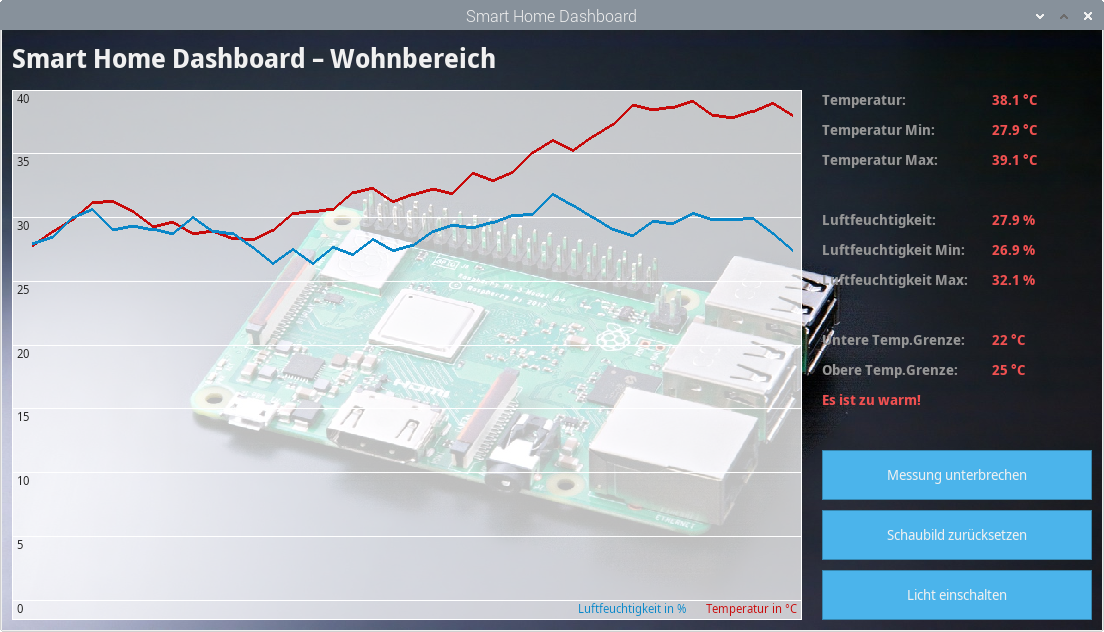
\includegraphics[width=\textwidth]{03-python1/img/aufgabe-dashboard}

Bevor es losgehen kann, benötigen wir wieder einen kleinen Hardwareaufbau:

\begin{enumerate}
    \item Ein blaue LED an GPIO-Pin 14
    \item Eine rote LED an GPIO-Pin 15
    \item Ein Relais zum Schalten einer Dummy-LED an Pin 18
    \item Einen DHT11-Luftsensor an Pin 23
\end{enumerate}

Die blaue LED soll immer dann blinken, wenn die gemessene Temperatur unter
einem bestimmten Grenzwert liegt. Entsprechend soll stattdessen die rote LED
blinken, wenn die Temperatur über einem zweiten, höheren Grenzwert liegt.
Die LEDs sollen somit also anzeigen, ob die Temperatur innerhalb des
\glqq{}Wohlfühlbereichs\grqq{} des Anwenders liegt. \smiley{} Das Relais hingegen
soll eigentlich die Zimmerbeleuchtung ein- und ausschalten. Um dies zu simulieren,
verwenden wir ebenfalls eine LED im Arbeitsstromkreis des Relais.

\bigskip
\teilaufgabe
Laden Sie sich nun von Moodle den Quellcode zur dieser Aufgabe runter und
entpacken Sie diesen auf dem Raspberry Pi. Anschließend öffnen Sie eine Konsole
und geben folgenden Befehl ein (ohne das Dollarzeichen):

\begin{verbatim}
$ sudo rpasi-config
\end{verbatim}

Im daraufhin erscheinenden Menü wählen Sie folgende Menüpunkte aus, um den
OpenGL-Grafiktreiber des Raspberry Pi zu aktivieren und somit ein Flimmern des
Programmfensters zu vermeiden. Danach starten Sie den Raspberry Pi neu.

\begin{itemize}
    \item Advanced Options → GL Driver → GL (Full KMS)
    \item Advanced Options → Compositor → Yes
\end{itemize}

Anschließend öffnen Sie die vorinstallierte \textbf{Thonny Python IDE},
wechseln in den \textbf{Regular Mode} (falls noch nicht geschehen) und öffnen
folgenden Menüpunkt:

\begin{itemize}
    \item Tools → Manage Packages…
\end{itemize}

Dort installieren Sie dann die Bibliothek \texttt{Adafruit-DHT} zur Ansteuerung
des DHT11-Luftsensors. Danach kann es mit der Aufgabe beginnen.

\bigskip
\teilaufgabe
Der Hauptteil des Programms befindet sich in der Klasse \texttt{Main} in der
gleichnamigen Datei \texttt{main.py}. Dort sind bereits mehrere Variablen mit
den Namen \texttt{self\-.led\_\-too\_\-cold}, \texttt{self\-.led\_\-too\_\-hot}
und so weiter für die einzelnen LEDs definiert. Schauen Sie sich zunächst die
dahinter stehende Klasse \texttt{Switch\-Output\-Device} an und versuchen Sie
herauszufinden, welche Methoden Sie zum Ein- und Ausschalten der LEDs bietet:

{
    \renewcommand{\arraystretch}{2.5}
    \medskip

    \begin{tabular}{p{0.2\textwidth}p{.8\textwidth}}
        LED einschalten: & \rule{20em}{1pt} \\
        LED ausschalten: & \rule{20em}{1pt} \\
        LED blinken:     & \rule{20em}{1pt} \\
    \end{tabular}

    \medskip
}

Bauen Sie entsprechende Methodenaufrufe in die \texttt{Main}-Klasse ein, um
die blaue LED blinken zu lassen, wenn die Temperatur zu kalt ist und die rote
LED, wenn die Temperatur zu warm ist. Achten Sie dabei aber darauf, dass stets
nur eine der beiden LEDs blinken soll.

Zunächst werden Sie das Blinken nur in der Konsolenausgabe der Anwendung sehen.
Denn die entsprechenden GPIO-Aufrufe zum Ein- oder Ausschalten des GPIO-Ausgangs
fehlen in der Klasse \texttt{Switch\-Output\-Device} noch. Nehmen Sie sich
hierfür die Beispielquellcodes aus dem Kapitel \glqq{}Hardwaredesign\grqq{}
zur Vorlage und erweitern Sie die Klasse so, dass der jeweilige GPIO-Pin im
Konstruktor als Auskunft konfiguriert und an der richtigen Stelle weiter unten
ein oder aus geschaltet wird.

\bigskip
\teilaufgabe
Bis hierhin nutzt die Anwendung noch nicht den richtigen DHT11-Luftsensor zur
Ermittlung der Temperatur- und Feuchtigkeitswerte. Stattdessen wird im Konstruktor
der Klasse \texttt{Main} ein \texttt{DHT11\-Mock\-Sensor}-Objekt erzeugt, das den
Sensor (mehr schlecht als recht) nur simuliert. Tauschen Sie das Objekt gegen eine
Instanz der Klasse \texttt{DHT11\-Sensor} aus, um echte Messwerte zu erhalten.

Allerdings müssen Sie die Klasse noch zu Ende programmieren. Schauen Sie sich an,
wie in der Klasse \texttt{DHT11\-Mock\-Sensor} das periodische \glqq{}Auslesen\grqq{}
der Sensordaten realisiert wurde und übernehmen Sie diese Lösung in die Klasse
\texttt{DHT11\-Sensor}. Schlüssel ist dabei die Methode \texttt{tick()}, die
mehrmals pro Sekunde vom Hauptfenster aufgerufen wird und dabei jedes mal prüft,
ob genügend Zeit seit der letzten Messung vergangen ist. Anstatt jedoch zufällige
Kennzahlen zu würfeln, müssen Sie den am Pi angeschlossen DHT11-Sensor mit Hilfe
des \texttt{Adafruit\_\-DHT}-Moduls ansprechen. Auch hierbei helfen Ihnen die
Codebeispiele aus dem Kapitel \glqq{}Hardwaredesign\grqq{} weiter.

\bigskip
\teilaufgabe
Zum Schluss sollen die gemessenen Sensorwerte in einer CSV-Datei mit dem Namen
\texttt{iot\--dashboard.csv} im Home-Verzeichnis des Benutzers protokolliert
werden. Legen Sie hierfür im Verzeichnis \texttt{logfile} eine neue Quelldatei
mit einer von \texttt{Data\-Logger} angeleiteten Klasse an, die bei jedem
Aufruf der Methode \texttt{log\_\-values()} eine neue Zeile in die CSV-Datei
schreibt. Die neue Klasse müssen Sie dann in \texttt{Main} an den entsprechenden
Stellen aufrufen. Als Hilfestellung schlagen Sie hierfür die Dokumentation des
in der Python-Bibliothek enthaltenen \texttt{csv}-Moduls nach.


%===============================================================================
\clearpage
\LoesungHeader
%===============================================================================

%-------------------------------------------------------------------------------
\loesung{Allgemeine Fragen über Python}
%-------------------------------------------------------------------------------
\teilaufgabe
Betriebssystem mit verfügbarer Python-Laufzeitumgebung: Alle. Die Liste wurde
ein zu eins von der Python-Downloadseite übernommen.

\begin{center}
    \begin{tabular}{p{.2\textwidth}p{.2\textwidth}p{.2\textwidth}}
        $\blacksquare$ Linux &
        $\blacksquare$ macOS &
        $\blacksquare$ Windows \\

        $\blacksquare$ Solaris &
        $\blacksquare$ OS390 &
        $\blacksquare$ zOS \\

        $\blacksquare$ iOS &
        $\blacksquare$ VMS &
        $\blacksquare$ HP-UX \\
    \end{tabular}
\end{center}

\bigskip
\teilaufgabe
Art der Kompilierung von Python-Programmen:

\begin{itemize}
    \renewcommand{\labelitemi}{$\blacksquare$}
    \item Die Art der Ausführung hängt von der verwendeten Python-Implementierung
    ab. Die auf \texttt{www.python.org} angebotene Referenzimplementierung nutzt
    einen mehr oder weniger einfachen Interpreter. Es gibt aber auch Implementierungen
    auf Basis eines Just-In-Time-Compilers oder für die Java Virtual Machine.
\end{itemize}

\teilaufgabe
Eigenheiten der Python-Syntax:

\begin{itemize}
    \renewcommand{\labelitemi}{$\blacksquare$}
    \item Python besitzt eine weitgehend eigene Syntax, die nicht von anderen
    Sprachen wie C oder C++ beeinflusst wurde.
\end{itemize}

\teilaufgabe
Programmierparadigmen in Python:

\begin{itemize}
    \renewcommand{\labelitemi}{$\blacksquare$}
    \item Python unterstützt mehrere Programmierparadigmen, genau wie C++.
\end{itemize}

\teilaufgabe
Inhalte von PEP8 und PEP20:

\begin{itemize}
    \renewcommand{\labelitemi}{$\blacksquare$}
    \item Einen Styleguide und Tipps für saubere Python-Programme
\end{itemize}

\teilaufgabe
Bedeutung des \glqq{}Duck Typing\grqq{} in Python:

\begin{itemize}
    \renewcommand{\labelitemi}{$\blacksquare$}
    \item Variablen werden nicht deklariert sondern entstehen durch ihre erste Zuweisung.
    \item Ob ein Objekt an einer bestimmten Stelle aufgerufen werden kann, entscheidet sich erst zur Laufzeit,
    wenn der Aufruf tatsächlich ausgeführt werden soll.
    \item Die Prüfung, die dabei stattfindet, bezieht sich allerdings nur auf das Vorhandensein
    gleichnamiger Methoden oder Attribute.
    \item Das heißt, ein Objekt kann ein anderes Objekt selbst dann ersetzen,
    wenn sie keine gemeinsame Basisklasse besitzen.
\end{itemize}

\clearpage

%-------------------------------------------------------------------------------
\loesung{Quellcode vervollständigen}
%-------------------------------------------------------------------------------
\teilaufgabe
Prüfung mehrerer Bedingungen:

\begin{Verbatim}[gobble=4]
    temperature = sensor.read_temperature()                 # Temperatur
    humidity = sensor.read_humdity()                        # Luftfeuchtigkeit

    if temperature >= 28 and humidity >= 70:                # Beides muss zutreffen
        print("Das reinste Tropenwetter hier!")
    elif temperature >= 25:
        print("Echt schönes Wetter heute.")
    elif temperature >= 18:
        print("Herrliches Frühlingswetter.")
    else:
        print("Wann wird es endlich wieder Sommer?")
        print("So wie es früher einmal war.")

\end{Verbatim}

%\bigskip
\teilaufgabe
Zugriff auf Dictionaries und Listen:

\begin{Verbatim}[gobble=4]
    backend_server = {
        "proto": "HTTPS",
        "host":  "backend.example.com",
        "port":  "8443",
        "path":  "/sensor/dht11/"
    }

    distance_meters = [8, 7, 5.5, 4, 3.8, 3.4, 3.1, 2.8, 2.5, 1]

    print("Hostname:     " + backend_server["host"])
    print("Port:         " + backend_server["port"])
    print("Erster Wert:  " + str(distance_meters[0]))
    print("Zweiter Wert: " + str(distance_meters[1]))
    print("Letzter Wert:"  + str(distance_meters[9]))

    // Besser
    print("Letzter Wert:"  + str(distance_meters[-1]))
\end{Verbatim}

\bigskip
\teilaufgabe
Definition einer Funktion und Aufruf derselben bei Programmstart:

\begin{Verbatim}[gobble=4]
    import sys

    def show_main_window(width, height):
        wnd = MainWindow(width, height)
        wnd.show()
        return 0

    if __name__ == "__main__":
        sys.exit(show_main_window())
\end{Verbatim}

\teilaufgabe
Ausnahmen abfangen und behandeln:

\begin{Verbatim}[gobble=4]
    def read_single_sensor_value():
        try:
            sensor.init()
            value = sensor.read_value()
        except HardwareAccessError:
            # Fehler hier behandeln …
            pass
        finally:
            # Hardware in jedem Fall schließen, selbst bei Fehlern zuvor
            sensor.close()
\end{Verbatim}

\teilaufgabe
Klassen definieren und instantiieren:

\begin{Verbatim}[gobble=4]
    class DHT11Sensor(HardwareDevice):
        """
        Diese Klasse ermöglicht den Zugriff auf einen DHT11-Sensor zur Ermittlung
        von Temperatur und Luftfeuchtigkeit.
        """

        def __init__(self, gpio_pin):
            """
            Konstruktor
            """
            self._gpio_pin = gpio_pin

        def read_values(self):
            """
            Auslesen eines Sensorwerts:
            """
            return (25, 30)     # TODO

        def close(self):
            """
            Hardwarezugriff schließen
            """
            pass                # TODO

    sensor = DHT11Sensor(27)
    temperature, humidity = sensor.read_values()
    print("Temperatur: " + temperature)
    print("Luftfeuchtigkeit: " + humidity)
\end{Verbatim}

%-------------------------------------------------------------------------------
\loesung{Fehler korrigieren}
%-------------------------------------------------------------------------------
\teilaufgabe
Bereinigung sämtlicher Syntaxfehler (mindestens 30 Stück, je nachdem wie man zählt):

\begin{Verbatim}[gobble=4]
    import os, sys, time
    from sensors import DHT11Sensor

    class UserInterface(Application):
        def __init__(self, w, h):
            super().__init__()
            self.window = MainWindow(w, h)
            self.window.set_title("IoT-Anwendung")

        def show(self):
            self.window.show()
            self.window.set_close_db(self.close_cb)
            return 0

        def close_cb(self, window):
          self.window.close()

    if __name__ == "__main__":
         ui = UserInterface()
         sys.exit(ui.show())
\end{Verbatim}

\teilaufgabe
Bereinigung der semantischen Fehler.

\begin{Verbatim}[gobble=4]
    values = []
    sensor = DHT11Sensor()                       # Klammern für Konstruktoraufruf

    try:                                         # try/except um die Schleife herum
        while True:
            temperature = sensor.read_temp()     # Klammern für Methodenaufruf
            values.append(temperature)
            sum = 0
            count = 1

            for value in values:
                sum += value                     # += für Zuweisung
                count += 1                       # Falsche Einrückung

            print("Gemessene Temperatur: " + temperature)
            print("Durchschnittliche Temperatur: " + sum / count)
    except KeyboardInterrupt:
        print("Auf wiedersehen!")
        print("Programm beendet sich nun.")
\end{Verbatim}

%-------------------------------------------------------------------------------
\loesung{Erste Schritte mit Python}
%-------------------------------------------------------------------------------
Hierzu gibt es keine Musterlösung. \smiley

%-------------------------------------------------------------------------------
\loesung{Smart Home Dashboard}
%-------------------------------------------------------------------------------
Den Quellcode der Musterlösung finden Sie auf Moodle.
